\documentclass[a4paper,11pt]{report}
\usepackage[T1]{fontenc}
\usepackage[utf8]{inputenc}
\usepackage[english]{babel}
\usepackage{lmodern}
\usepackage{amsmath, systeme}
\usepackage{amsfonts}
\usepackage{amssymb}
\usepackage{amsthm}
\usepackage{graphicx}
\usepackage{color}
\usepackage{xcolor}
\usepackage{url}
\usepackage{theorem}
\usepackage{textcomp}
\usepackage{listings}
\usepackage{hyperref}
\usepackage{parskip}
\usepackage{svg}
\usepackage{epigraph}
\usepackage{amssymb}
\usepackage{graphicx}
\usepackage[ligature, inference]{semantic}
\usepackage{float}   % For H placement
\lstset{
	basicstyle=\ttfamily\small,  % Use a smaller monospace font
	lineskip=-2pt,               % Reduce the vertical space between lines
	breaklines=true              % Allow long lines to wrap
}

\usepackage{semantic}

\title{Project report for Languages, Compilers and Interpreters}
\author{Dario Bekic}
\date{\today}

\begin{document}

\maketitle
\tableofcontents

\begin{abstract}
This report includes the necessary design explanations for the A.Y. 2024/2025 project of the Languages, Compilers and Interpreters at Università di Pisa.
The full project can be found on GitHub visiting this \href{https://github.com/wuacs/unipi-lci/tree/main/project}{link}.
The project's main goal is to design and implement aspects of programming languages in OCAML. Two main languages were developed: \verb|miniimp| and \verb|minifun|. For \verb|minifun|, it was developed a typed version \verb|minityfun|. For those languages we first define their ASTs and evaluation functions, then, using OCamllex and Menhir we develop a lexer and a parser for those languages. The formal, ambiguous, grammars can be found \href{https://lceragioli.github.io/pages/Slides/semantics.pdf}{here} and \href{https://lceragioli.github.io/pages/Slides/types.pdf}{here} and the explanations of how the ambiguities were resolved is detailed in \autoref{chap:parsing}.
\end{abstract}

\section{MiniFun}
\label{Section::MiniFun}

MiniFun is a simple untyped functional language. A parser was not implemented for MiniFun but instead for its typed counterpart. MiniFun is a single-module library which defines both its AST and an $\verb|eval_fun_ast|$ which takes a value of type $\verb|ast|$, representing a program written in MiniFun, and returns a element of type $\verb|value|$ which can be either a function, since we are in a functional language, or an integer or a boolean.
The run-time environment is a value of type $\verb|env|$ which is simply a map with strings as keys, so that we can keep track of variables.
One interesting thing of the evaluation function is that, if it fails to resolve a variable during its execution, (i.e. said variable was not initialized with a $\verb|Let|$ or $\verb|LetFun|$ construct) it fails.
 

\section{Minityfun}

MiniTyFun is a typed version of \hyperref[Section::MiniFun]{MiniFun}. 

\subsection{Missing Rules}

The only two rules which differ between MiniTyFun and MiniFun are the rules involving the typed constructs i.e. Anonymous function declaration 
\begin{figure}[H]
$\verb|LET FUN|$
\\
\[
\inference[]
{ 
	\Gamma[f \mapsto \tau \texttt{ -> } \tau'] \vdash t' \triangleright \tau''\quad
	\Gamma \vdash t \triangleright \tau'
}
{
	\begin{array}{c}
		\Gamma \vdash  \text{ letfun } f x:\tau = t \text{ in } t' \triangleright \tau''
	\end{array}
}
\]	
\end{figure}


$\verb|FUN|$
\\
\[
\inference[]
{ 
\Gamma \vdash t \triangleright \tau'
}
{
\begin{array}{c}
\Gamma \vdash  \text{ fun } x:\tau \texttt{ => } t \triangleright (\tau \rightarrow \tau')
\end{array}
}
\]

\section{Project Fragment 4 - Parsing}\label{chap:parsing}

\subsection{The negative conflict}

Since this conflict is of interest of both \verb|miniimp|'s and \verb|minifun|'s parsers we put it here and explain how we resolved it.
We do not repeat the statement of the problem, which can be found \href{https://lceragioli.github.io/pages/Slides/parsingErrataCorrige.pdf}{here}, only its solution implementation in Menhir.
In \verb|miniimp| the problem's solution is simply to adopt the convention specified \href{https://lceragioli.github.io/pages/Slides/parsingErrataCorrige.pdf}{here}, that is, our lexer is able to scan only naturals(\verb|natural| in the lexer specification) and the minus symbol(\verb|symbol|).
With \verb|minityfun|(and its untyped counterpart) we have the additional problem of function applications, because we need to distinguish the cases for an expression such \verb|factor - factor| which can be either interpreted as \verb|term (-term)| or \verb|term - term|. We decided to use the simple solution of wrapping the negative value in parenthesis.

\subsection{Miniimp's conflicts}

Each conflict is named with the type of conflict, i.e. SHIFT/REDUCE or REDUCE/REDUCE, together with the construct it mainly involves.
\begin{itemize}
    \item \textbf{SHIFT-REDUCE WHILE}: 
    \begin{lstlisting}
        WHILE bool_expr DO command

        State1:  command . SEQ command

        State2: WHILE bool_expr DO command .
    
        Lookahead symbol: SEQ
    \end{lstlisting}
\verb|State1| represents placing a sequence of commands in the body of the \verb|WHILE| construct.\\
\verb|State2| represents placing a \verb|;|, i.e. a \verb|SEQ| character, after a \verb|WHILE|, because the entire \verb|WHILE| expression could be reduced to a term.\\
\textbf{Solution}: adopt the C-like convention of having sequential commands refer to the same block with brackets as delimiters.

    \item \textbf{SHIFT-REDUCE IF}:
    \begin{lstlisting}
(S1) IF bool_expr THEN command ELSE command
                                    command . SEQ command

(S2) IF bool_expr THEN command ELSE .
    \end{lstlisting}
    \verb|State1| represents extending the \verb|ELSE|'s body with a sequence of commands\\
    \verb|State2| represents placing a command after an IF.\\
    \textbf{Solution}: 
    Similarly to the problem of \verb|SHIFT-REDUCE WHILE| we need to be explicit to how commands are grouped together in constructs which induce a block. \textbf{Note}: the branch of the \verb|THEN| does not present this ambiguity, however for uniformity we decided to follow this convention for the \verb|THEN| branch too: a sequence of instruction belongs to the nearest \verb|THEN| block only if they are wrapped in brackets, otherwise only the first instruction belongs to the \verb|THEN| and, since we do not have a \textit{short} conditional statement, the parsing fails. 
    
    \item \textbf{SHIFT-REDUCE Sequencing}
    
    \begin{lstlisting}
    State1:
    command SEQ command 
                command . SEQ command 

    State2:
    command SEQ command // lookahead token appears
    command SEQ command .
    \end{lstlisting}
    
    The problem is that we do not spec\lstset{
  language=Python, % Specify the language for syntax highlighting
  basicstyle=\ttfamily\small, % Set the font style and size
  captionpos=b, % Position of the caption (b for below, t for top)
}ify associativity: we choose to do it in the typical left associative way.\\
    \textbf{Solution}: we will give left-associativity using the Menhir-specific directive:\\
    \verb|%left SEQ|   
    
    \item \textbf{SHIFT-REDUCE Arithmetic}\\
    The following conflict is the  \\
    Thus, we will provide only one example:
        
    \begin{lstlisting}
arit_expr MINUS arit_expr 
                arit_expr . PLUS arit_expr 
                
arit_expr PLUS arit_expr // lookahead token appears
arit_expr MINUS arit_expr .
    \end{lstlisting}
    
    Menhir tells us that, while having as a symbol of look-ahead \verb|PLUS|, we could be shifting
    or immediately reduce the \verb|MINUS| operation.
    Thus we will give left associativity to arithmetic(and boolean) tokens with the exception for the \verb|NOT| operator which will be given higher precedence.
\end{itemize}

\subsection{Minityfun's conflicts}

Conflicts found:

\begin{itemize}
    \item \textbf{SHIFT-REDUCE (LET)FUN context}\\
    Menhir gives the following conflict:
    \begin{lstlisting}

    term PLUS term // lookahead token appears
    LETFUN VAR VAR TYPE_SEP typing term IN term . 

    LETFUN VAR VAR TYPE_SEP typing term IN term 
                                           term . PLUS term 
    \end{lstlisting}
    Clearly we want that the part \verb|... IN term PLUS term| to mean that in the context of \verb|LETFUN| (or \verb|FUN|) we have the sum of two terms, not that we sum the \verb|LETFUN| term with another one. \\
    \textbf{Solution}: redesign the grammar so that we give higher precedence to the arithmetic and boolean operators(\verb|PLUS, AND, OR|...) by creating the non-terminals \verb|operation| and \verb|basic_term|. A \verb|term| can then rewrite itself to an operation which is a sequence of binary operators whose base production is \verb|operation -> basic_term|. \verb|basic_term| is either a literal, a variable or a new \verb|term| but wrapped in parentheses so that it gets precedence.
    
\item \textbf{SHIFT-REDUCE Application}\\
    An application is formally defined as \verb|t t|, thus clearly we have the problem of either shifting 
    a term in a \verb|FUN| or \verb|LETFUN| \textit{or} reducing the term so that we can use it as a term in an application. This is similiar to the problem of the previous point. \\
    \textbf{Solution}: a simple solution would be to incorporate the application production in the \verb|operation| non-terminal productions, as function application can be seen as a binary operations, and the already defined left associativity for operators well suits the currying ability of our function applications, meaning that \verb|f x y z| is interpreted as \verb|((f x) y ) z|.

\end{itemize}

\section{Project Fragment 5 - CFGs}

For the Control-Flow Graph module I followed the maximal block approach. That is, if two blocks do not differ in the branches or jumps they permit, and they are in program order, then the two blocks should be unified in one single block.
\\
Our CFG-building function for $\verb|miniimp|$ maintains the invariant that the initial node(called $\verb|entry|$) of any sub-CFG shall not have any incoming arc and the last(called $\verb|exit|$) shall not have any outgoing arc.
Consider the $\verb|miniimp|$ program in listing 3.1. The CFG, rendered by using the file produced by function $\verb|cfg_to_dot|$, using the \href{https://graphviz.org/download/}{graphiz} package, can be seen in figure \ref{fig:cfg:fibonacci}.
Notice how there are 3 SKIP nodes which could be merged, but for run-time parsing they are kept separate:
\begin{itemize}
  \item Each $\verb|while|$ construct generates a new end node because the end node must not have any outgoing arc, thus the block containing 4 assignments cannot be regarded as final.
  \item Each $\verb|if|$ construct generates a final block as it has no way of knowing if the intermediate blocks have generated final skip blocks, as in the case of a $\verb|while|$ construct, or they are simply one block of instructions, like a sequence of instruction would generate.
  \item The $\verb|SKIP|$-only block coming out of the green block is a SKIP block simply because the program has one such instruction in the else branch of the $\verb|if|$ construct.
However sequences of blocks are correctly compacted in one block: in the green block we have compacted the instructions generated by sequencing and the guard generated by the $\verb|if|$ construct.
\end{itemize}
\newpage

\begin{lstlisting}[caption={Fibonacci in miniimp}]
def main with input in output out as
    x := in;
    out := 0;
    if not x < 2 then 
        x := x - 1;
        out := 1;
        second := 0;
        while not x < 2 do (
            temp := out;
            out := out + second;
            x := x - 1;
            second := temp
        )
    else ( skip );
    skip
\end{lstlisting}

\begin{figure}
  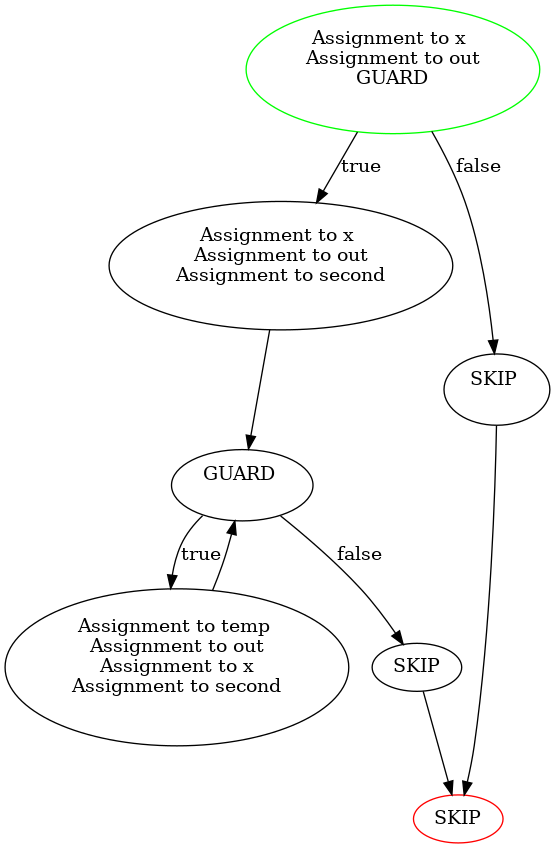
\includegraphics[width=\linewidth]{./report_resources/fibonacci.png}
  \label{fig:cfg:fibonacci}
  \caption{CFG for Fibonacci's program}
\end{figure}

\section{Analyses}

We implemented two data flow analyses for the Intermediate Representation of the Control Flow Graph of MiniRISC: the defined variable analysis, implemented by the module $\verb|defined_analysis|$ module and the liveness analyis implemented by module $\verb|liveness_analysis|$.
We defined utility functions on the Control Flow Graph which may be used by different data flow analyses, such as $\verb|get_bottom|$ which returns the set of all registers defined in our Control Flow Graph, which is used, for example, when initializing the $\verb|LIVE_IN and LIVE_OUT|$ sets at the start of the liveness analysis.

\section{Target Code Generation}

\section{How to use}

The objective of the laboratory was to design and implement the following components:

\begin{itemize}
	\item A MiniFun interpreter 
	\item A MiniTyFun interpeter and parser
	\item A MiniImp interpreter and parser
	\item A MiniImp compiler to MiniRISC which needs to provide two options: one for optimizing the number of registers used in the generated code, and one for performing a static analysis to check whether every variable was initialized before use. 
\end{itemize}

Thus we provide the following sections for explaining how to test each component.

\subsection{MiniFun interpreter}

While in the project roots


\end{document}

